% CAP description for Menu Bar
\begin{itemize}
\item A \bxname{menu bar} is the component typically 
found at the top of an application window.
\item It typically contains menus such as  ''File'', ''Edit'',
  ''Help'', etc.
\end{itemize}

\begin{figure}
\begin{center}
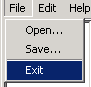
\includegraphics{PS/Menu}
\caption{Menu Bar}
\label{menu}
\end{center}
\end{figure}

Because the forward slash (/) is a special symbol for menus, if you want to use a slash as part of your parameter value, you have to mask it. See the section later in this document \bxpref{specialchar} for more details. 

\textbf{Mapping menu bars}

Menu bars do not need to be mapped in the \gdomm{} as they are automatically found during test execution.

\bxtipp{Actions on menus are not supported in the HTML toolkit.}
